\section{Clustering using a pre-trained model}

As previously discussed in section \ref{sec:architectures} we use the VGG16 pre-trained network as a baseline for the clustering performance also. We begin by considering a classical K-means approach to clustering. However, the output from the VGG16 network is very high dimensional at some $\sim 8e3$ floats. One of the primary concerns is then the curse of dimensionality, where the ratio of distances goes to one with increasing dimensionality (\cite{Aggarwal}). However, one of the central caveats to this finding is that the elements are uniformly distributed in the space. It is then possible that all the class information lies in some sub-space of the latent data. To investigate this we perform clustering analysis using the full representation, and using the $10^2$ principal components only. 

\subsection{K-means}

We begin by investigating the K-means clustering algorithm using the $10^2$ primary principal components on all datasets. As in the previous chapter the VGG16 model is pre-trained on the imagenet dataset creating a set of vectors $\mathbf{x} \in \mathcal{R}^{8192}$. To cluster we use \lstinline{scikit-learn} implementation of the K-means algorithm, with default parameters (\cite{Pedregosa2011}). The results of the clustering runs are included in table \ref{tab:clstr_vgg}. We observe  that we are able to attain near perfect clustering on simulated data, and that there is a sharp decline in performance as we add noise by moving to the filtered and full datasets. 

\begin{table}[H]
\centering 
\caption[K-means on pre-trained model]{K-means clustering results on AT-TPC event data. We observe that the performance goes predictably down with the amount of noise in the data.}\label{tab:clstr_vgg}
\begin{tabular}{lll}
\toprule
{} & Accuracy &   ARI \\
\midrule
Simulated &     0.97 &  0.89 \\
Filtered  &     0.74 &  0.39 \\
Full      &     0.59 &  0.17 \\
\bottomrule
\end{tabular}

\end{table}


In addition to the performance measures reported in table \ref{tab:clstr_vgg} it is interesting to observe which samples are being wrongly assigned. We achieve this by tabulating the assignments of samples relative to their ground truth labels. From these tables we can infer which classes are more or less entangled with the others. One table for each dataset is in figure \ref{fig:clster_confmat}. We observe that the proton class is consistently the most pure cluster. Purity is inferred from observing how evenly the columns are spread for each row, and how much spread there is in the column we infer belongs to that class. For example, consider the row corresponding to the proton class in \ref{fig:clster_confmat}. The column corresponding to the largest entry in the proton row has very few other predicted classes. From this we infer that the proton class is clearly distinct from the others. 

\begin{figure}
\centering
	\subfloat{
	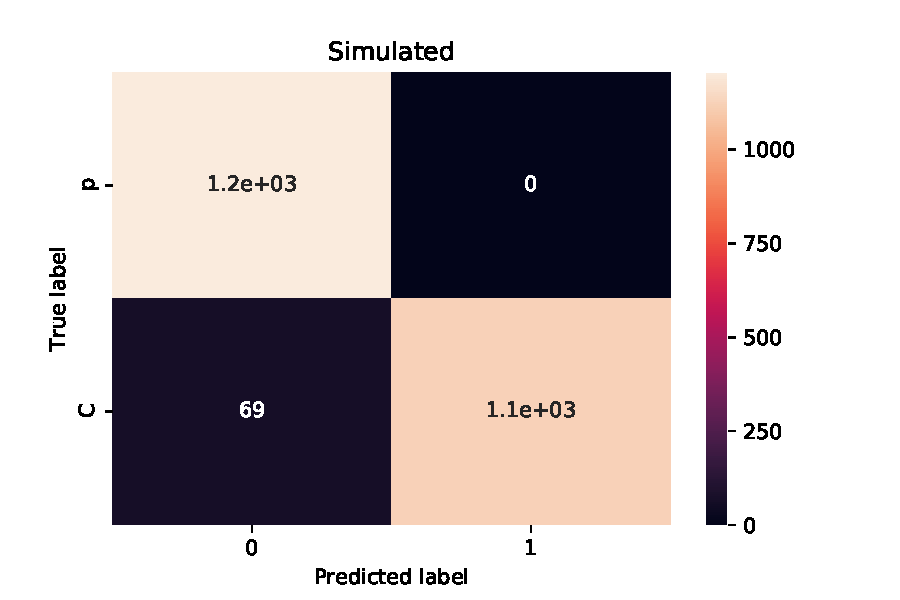
\includegraphics[width=0.35\textwidth]{./plots/Simulatedconf_mat.pdf}

}
	\hspace{-1cm}
	\subfloat{
	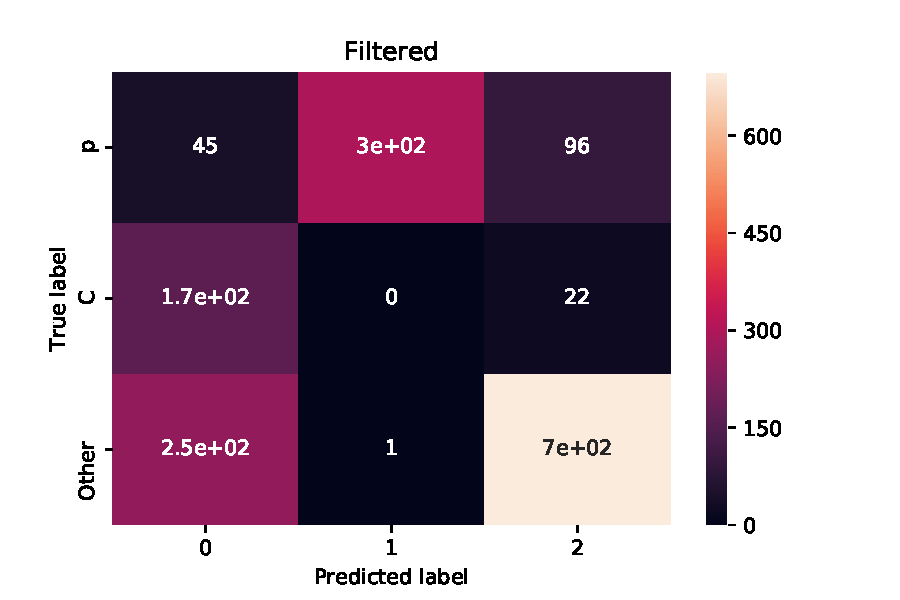
\includegraphics[width=0.35\textwidth]{plots/Filteredconf_mat.pdf}
}
	\hspace{-1cm}
	\subfloat{
	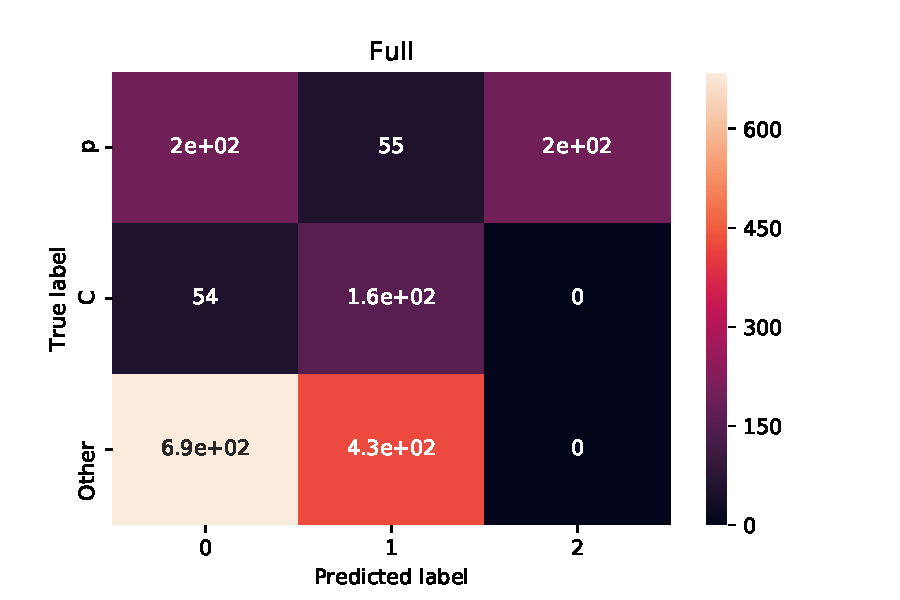
\includegraphics[width=0.35\textwidth]{plots/Fullconf_mat.pdf}
}
\caption[Pre-trained network - confusion matrices]{Confusion matrices for the K-means clustering of simulated, filtered and full AT-TPC events. The true labels indicate samples belonging to the p (proton), C (carbon), or other classes. }\label{fig:clster_confmat}
\end{figure}

We repeat this analysis using a PCA dimensionality reduction on the latent space of the VGG16 model. This is done to estimate to what degree the class separating information is encoded in the entirety of the latent space, or in some select regions. The results from the PCA analysis were virtually identical to the results sans the PCA, and so we omit them for brevity. 